% Options for packages loaded elsewhere
\PassOptionsToPackage{unicode}{hyperref}
\PassOptionsToPackage{hyphens}{url}
%
\documentclass[
]{book}
\usepackage{lmodern}
\usepackage{amssymb,amsmath}
\usepackage{ifxetex,ifluatex}
\ifnum 0\ifxetex 1\fi\ifluatex 1\fi=0 % if pdftex
  \usepackage[T1]{fontenc}
  \usepackage[utf8]{inputenc}
  \usepackage{textcomp} % provide euro and other symbols
\else % if luatex or xetex
  \usepackage{unicode-math}
  \defaultfontfeatures{Scale=MatchLowercase}
  \defaultfontfeatures[\rmfamily]{Ligatures=TeX,Scale=1}
\fi
% Use upquote if available, for straight quotes in verbatim environments
\IfFileExists{upquote.sty}{\usepackage{upquote}}{}
\IfFileExists{microtype.sty}{% use microtype if available
  \usepackage[]{microtype}
  \UseMicrotypeSet[protrusion]{basicmath} % disable protrusion for tt fonts
}{}
\makeatletter
\@ifundefined{KOMAClassName}{% if non-KOMA class
  \IfFileExists{parskip.sty}{%
    \usepackage{parskip}
  }{% else
    \setlength{\parindent}{0pt}
    \setlength{\parskip}{6pt plus 2pt minus 1pt}}
}{% if KOMA class
  \KOMAoptions{parskip=half}}
\makeatother
\usepackage{xcolor}
\IfFileExists{xurl.sty}{\usepackage{xurl}}{} % add URL line breaks if available
\IfFileExists{bookmark.sty}{\usepackage{bookmark}}{\usepackage{hyperref}}
\hypersetup{
  pdftitle={İstatistiksel Kalite Kontrol},
  pdfauthor={Dr.~Busenur Kızılaslan},
  hidelinks,
  pdfcreator={LaTeX via pandoc}}
\urlstyle{same} % disable monospaced font for URLs
\usepackage{longtable,booktabs}
% Correct order of tables after \paragraph or \subparagraph
\usepackage{etoolbox}
\makeatletter
\patchcmd\longtable{\par}{\if@noskipsec\mbox{}\fi\par}{}{}
\makeatother
% Allow footnotes in longtable head/foot
\IfFileExists{footnotehyper.sty}{\usepackage{footnotehyper}}{\usepackage{footnote}}
\makesavenoteenv{longtable}
\usepackage{graphicx,grffile}
\makeatletter
\def\maxwidth{\ifdim\Gin@nat@width>\linewidth\linewidth\else\Gin@nat@width\fi}
\def\maxheight{\ifdim\Gin@nat@height>\textheight\textheight\else\Gin@nat@height\fi}
\makeatother
% Scale images if necessary, so that they will not overflow the page
% margins by default, and it is still possible to overwrite the defaults
% using explicit options in \includegraphics[width, height, ...]{}
\setkeys{Gin}{width=\maxwidth,height=\maxheight,keepaspectratio}
% Set default figure placement to htbp
\makeatletter
\def\fps@figure{htbp}
\makeatother
\setlength{\emergencystretch}{3em} % prevent overfull lines
\providecommand{\tightlist}{%
  \setlength{\itemsep}{0pt}\setlength{\parskip}{0pt}}
\setcounter{secnumdepth}{5}
\usepackage{booktabs}
\usepackage[]{natbib}
\bibliographystyle{apalike}

\title{İstatistiksel Kalite Kontrol}
\author{Dr.~Busenur Kızılaslan}
\date{2020-10-12}

\begin{document}
\maketitle

{
\setcounter{tocdepth}{1}
\tableofcontents
}
\hypertarget{uxf6n-bilgi}{%
\chapter{Ön Bilgi}\label{uxf6n-bilgi}}

Ders notları temelde \emph{IST3032 İstatistiksel Kalite Kontrol} dersine kaynaklık etmesi amacıyla tasarlanmış olup konu çerçevesinde kendini geliştirmek isteyen herkesin faydalanabilmesi hedeflenmiştir.

Ders dili Türkçe'dir. Bu bakımdan genel anlatımda Türkçe kullanılacaktır. Literatürü rahat takip edebilmeniz ve terim karmaşası yaşamamanız adına temel terim kısaltmaları orijinal haliyle kullanılacaktır (Kısaltmalar bölümünde hem Türkçe hem İngilizce açılımları bulabilirsiniz). Referans verilen kaynaklardan faydalanabilmeniz ve ders sürecinde incelemeniz gereken makalelerde zorluk yaşamamanız adına İngilizce eksikliğinizi gidermeniz önerilir.

Ders uygulamaları R programlama dili ile gerçekleştirilecek olup ödev uygulamalarınızı bu programlama dili ile hazırlamanız istenecektir, bu sebeple \emph{Bilgisayar III} ve \emph{Bilgisayar IV} ders notlarınızı gözden geçirmeniz faydalı olacaktır.

\textbf{İletişim adresi:} \href{mailto:busenur.sarica@marmara.edu.tr}{\nolinkurl{busenur.sarica@marmara.edu.tr}}

\textbf{Kaynaklar}

\begin{itemize}
\item
  \href{http://endustri.eskisehir.edu.tr/ipoyraz/TKY302/icerik/text\%20book_montgomery_6th\%20edition.pdf}{Introduction to Statistical Quality Control - Douglas C. Montgomery}
\item
  \href{http://www.diliev.com/Home/materiali/KHEA/referati/6812268-Statistical-Process-Control-eBook-VG.pdf}{Statistical Process Control - John S. Oakland}
\item
  İstatistiksel Kalite Kontrol Ders Notları - Erhan Öner
\item
  \href{http://auzefkitap.istanbul.edu.tr/kitap/endustrimuhlt_ue/istatistikselkalitekontrolu.pdf}{İstatistiksel Kalite Kontrol Ders Notları - Tuncay Özcan}
\end{itemize}

\hypertarget{hakkux131mda}{%
\section{Hakkımda}\label{hakkux131mda}}

2012 yılında Mimar Sinan G. S. Üniversitesi istatistik bölümünde lisans öğrenimimi tamamlamamın ardından 2014 yılı itibariyle Marmara Üniversitesi istatistik bölümünde araştırma görevlisi olarak göreve başladım. Eş zamanlı olarak başladığım yüksek lisans öğrenimimi yine Mimar Sinan G. S. Üniversitesi istatistik anabilim dalında tamamlarken artık çalışma alanım bulanık mantık (\href{https://en.wikipedia.org/wiki/Fuzzy_logic}{fuzzy logic}) olarak şekillenmişti. Bir buçuk yılda tamamladığım yüksek lisansın ardından farklı bakış açısı kazanma fikriyle yönümü Yıldız Teknik Üniversitesi'ne çevirdim. 2015 yılında istatistik bölümünde başladığım doktora öğrenimimi 2020 yılında yine bulanık mantık ile öngörü üzerine hazırladığım tezim ile tamamladım. Doktora öğrenimim sırasında İstanbul Teknik Üniversitesi endüstri mühendisliği bölümünden de çeşitli dersler alarak alanında uzman hocaların\footnote{\href{http://akademi.itu.edu.tr/kahramanc/}{Prof.~Dr.~Cengiz Kahraman}} bilgilerinden faydalanma imkanı buldum.

Akademik kariyer hedefiyle başlamadığım öğrenim yaşamımda ufku açık, aydınlık ve birikimli hocalarım yolumu bulmama yardımcı olmuştur. 2018 yılında Polonya'da gerçekleşen \href{http://www.linstat2018.put.poznan.pl/ysa.html}{International Conference on Trends and Perspectives in Linear Statistical Inference (LinStat'2018)} kapsamında sunduğum, doktora tezimin bir kısmından oluşan çalışma ile aldığım Young Scientists Awards ikincilik ödülü de yanlış yolda olmadığımı göstermiştir.

Üzerimde emeği olan herkese teşekkürlerimle!

\href{https://avesis.marmara.edu.tr/busenur.sarica}{\textbf{CV}}, \href{https://scholar.google.com.tr/citations?user=OKlYJEgAAAAJ\&hl=tr}{\textbf{Google Scholar}}, \href{https://www.linkedin.com/in/busenur-kızılaslan-795ab54a}{\textbf{Linkedin}}

\hypertarget{motivasyon}{%
\chapter{Motivasyon}\label{motivasyon}}

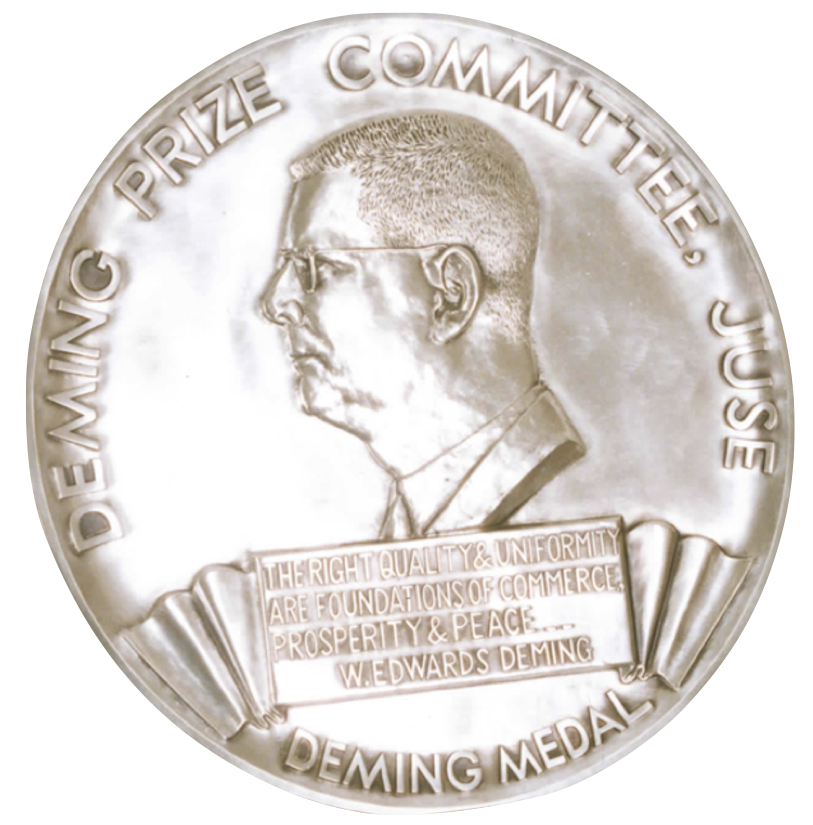
\includegraphics[width=11.29in]{/Users/busenursarica/Documents/GitHub/quality-control/images/dprize}

Kaliteyi kontrol etmek ve iyileştirmek rekabet ortamında kazananı belirleyen faktör haline gelmiştir. Bu bakımdan doğru yürütülen bir kalite kontrol süreci başarının anahtarı olacaktır. Sürecin başarılı yürütülmesi ise ancak alanında uzman kişilerin önderliğinde mümkündür.

İstatistikçiler için olası bir çalışma alanı olan \emph{İstatistiksel Kalite Kontrol}, gelecekte sizlerden biri veya birilerinin de yöneleceği alan olabilir. Bu bakımdan ders kapsamındaki bilgileri özümsemek, uygulamaları kavramak önem arz etmektedir.

Dr.~W. Edwards Deming tarafından yazılmış, incelenmesi gereken makaleler;

\href{https://deming.org/wp-content/uploads/2020/06/On-The-Statisticians-Contribution-to-Quality-1987.pdf}{On the statistician's contribution to quality}

\href{https://deming.org/wp-content/uploads/2020/06/Some-Responsibilities-of-a-Statistician-1964.pdf}{Some responsibilities of the statistician}

\hypertarget{genel-bakux131ux15f}{%
\chapter{Genel Bakış}\label{genel-bakux131ux15f}}

Here is a review of existing methods.

\hypertarget{kalite-yuxf6netimi-temel-kavramlarux131}{%
\chapter{Kalite Yönetimi Temel Kavramları}\label{kalite-yuxf6netimi-temel-kavramlarux131}}

\hypertarget{kalite-kavramux131}{%
\section{Kalite Kavramı}\label{kalite-kavramux131}}

Kalite tanımı birçok farklı şekilde yapılabilir. Kalitenin sözlük anlamı \emph{mükemmeliyet derecesi} olmakla birlikte, ürün/hizmette mevcut olması istenen özellik veya özellikler, kalite tanımı için başlangıç noktası olarak seçilebilir. Kalitenin çok boyutlu ve doğası gereği göreceli yapısı ortak bir tanımdan ziyade farklı bakış açılarıyla geliştirilmiş kalite tanımlarını ortaya çıkarmıştır. Amerikan Kalite Derneği (ASQ); kaliteyi farklı tanımlamaların yapılabileceği öznel bir terim olarak tanımlamıştır.

\begin{itemize}
\tightlist
\item
  Kalite, gereksinimlere uygunluktur. (Crosby)
\item
  Kalite, kullanıma uygunluktur. (Juran)
\item
  Kalite, müşterinin şimdiki ve gelecekteki ihtiyaçlarını hedeflemektir. (Deming)
\item
  Kalite, müşteri beklentilerini karşılayacak ürün ve hizmetin pazarlama, mühendislik, imalat ve bakım aşamalarındaki karakteristiklerinin toplamıdır. (Feigenbaum)
\item
  Kalite, özelliklerin ve gereksinimleri yerine getirme derecesidir. (ISO 9000)
\item
  Kalite, mal ve hizmetlerde, özellikle gereksinimlere uydukları ve müşterileri tatmin ettikleri ölçüde mükemmelliği ifade eder. (ASQ)
\end{itemize}

Kalite değişkenlikle ters orantılıdır. Ürün/hizmetin önemli karakteristiklerindeki değişkenliğin azaltılması kaliteyi arttıracaktır.

Değişkenliğin kalite kontrol açısından önemini kavramak açısından bir örnek verelim. Amerika Birleşik Devletleri'ndeki bir otomobil şirketi, şanzıman üretimlerini hem yerli bir tesiste hem de Japon bir tedarikçi aracılığıyla gerçekleştirmektedir.

Garanti taleplerinin ve onarım maliyetlerinin analizi, sütun grafikte gösterilmiştir, Japon üretimi şanzımanın çok daha düşük maliyetlere sahip olmasıyla, iki üretim kaynağı arasında çarpıcı bir fark olduğu görülmektedir. Maliyet ve performanstaki bu farkın nedenini keşfetme çalışmasının bir parçası olarak, şirket her tesisten rastgele iletim örnekleri seçmiş, bunları parçalara ayırmış ve birkaç kritik kalite özelliğini ölçmüştür.

Kritik boyutların her iki dağılımı da hedef değerde ortalanmıştır. Bununla birlikte, Amerika Birleşik Devletleri'nde üretilen şanzımanlar için kritik özelliklerin dağılımı, spesifikasyonların genişliğinin yaklaşık\% 75'ini kaplar ve bu da çok az sayıda uygun olmayan birimin üretileceğini gösterir. Aslında tesis, şirket içinde genel kabul görmüş kalite anlayışına göre oldukça iyi bir kalite seviyesinde üretim yapmaktadır. Buna karşılık, Japon fabrikası aynı kritik özelliklerin spesifikasyon bandının sadece yaklaşık\% 25'ini kapladığı aktarımlar üretmiştir. Sonuç olarak, Japon yapımı şanzımanların kritik kalite özelliklerinde Amerika Birleşik Devletleri'nde üretilenlere kıyasla önemli ölçüde daha az değişkenlik mecvuttur.

Akla gelen ilk soru Japonlar bunu nasıl yaptı? Burada azalan değişkenlik, doğrudan daha düşük maliyetlere dönüşmüştür. Dahası, Japon yapımı şanzımanlar daha sorunsuz vites değiştirmiş, daha sessiz çalışmış ve genellikle müşteri tarafından yurt içinde üretilenlerden daha üstün olarak algılanmıştır. Daha az onarım ve garanti talebi, daha az yeniden çalışma ve boşa harcanan zaman, çaba ve paranın azaltılması anlamına gelmektedir. Dolayısıyla, \textbf{kalite gerçekten değişkenlikle ters orantılıdır.} Dahası maliyetle yakından ilişkilidir.

Japonlar bunu nasıl yaptı? Cevap, kalite kontrolün sistematik ve etkili kullanımında yatmaktadır.

Kalite, rakip ürün/hizmetlerin seçiminde en önemli tüketici karar faktörlerinden biri haline gelmiştir. Bu görüş, tüketicinin bir birey, bir endüstriyel kuruluş, bir perakende mağazası, bir banka veya finans kurumu veya bir askeri savunma programı olmasına bakılmaksızın yaygındır. Sonuç olarak, kaliteyi anlamak ve iyileştirmek, iş başarısı, büyüme ve rekabet gücü açısından önemlidir. Bu bakımdan kalitenin iyileştirilmesi ve genel iş stratejisinin ayrılmaz bir parçası haline getirilmesi başarının temel gereklerindendir.

\texttt{Kalite\ terminolojisinde\ ürün\ (product)\ hem\ ürün\ hem\ de\ hizmet\ anlamında\ kullanılmaktdır.}

\textbf{Kalite iyileştirme (quality improvement):} Proses ve ürünler açısından değişkenliğin azaltılması olarak tanımlanmaktadır. Fazla miktarda değişkenlik performansta kayıba (waste) neden olmaktadır, para kaybı, zaman kaybı veya enerji kaybı örnek olarak verilebilir. Kalite iyileştirmenin bir diğer tanımı da \emph{kaybın azaltılması (reduction of waste)} olarak yapılabilir.

\hypertarget{kalite-boyutlarux131}{%
\section{Kalite Boyutları}\label{kalite-boyutlarux131}}

Kalitenin çok boyutlu yapısı farklı kalite tanımlarının ortaya çıkmasına neden olmuştur. Garvin (1987), kalitenin sekiz boyutunu şöyle tanımlamaktadır.

\textbf{1. Performans:} Temel ürün özellikleri

\textbf{2. Güvenilirlik:} Kullanım ömrü içerisindeki performans tutarlılığı

\textbf{3. Dayanıklılık:} Yararlı kullanım ömrü

\textbf{4. Hizmet:} Kullanım ömrü içerisinde problem ve şikayetlerin çözümü

\textbf{5. Estetik:} Duyulara seslenebilme özelliği

\textbf{6. Özellikler:} Öne çıkmayı sağlayan ikincil karakteristikler

\textbf{7. İtibar:} Geçmiş performans ve algılanan kalite

\textbf{8. Uygunluk:} Endüstri standartlarına uygunluk

\begin{verbatim}
Kalite çalışmalarında tüm boyutlar dikkate alınmalıdır.
\end{verbatim}

\hypertarget{kalite-muxfchendislik-terminolojisi}{%
\section{Kalite Mühendislik Terminolojisi}\label{kalite-muxfchendislik-terminolojisi}}

Her ürün, kullanıcının veya tüketicinin kalite göstergesi olarak tanımladığı bir takım unsurlara sahiptir. Bu unsurlara genellikle kalite karakteristikleri denir. Aynı zamanda kalite için kritik (critical to quality (CTQ)) karakteristikler olarak da tanımlanmaktadır. Kalite karakteristikleri birkaç türde olabilir:

\begin{itemize}
\item
  \textbf{Fiziksel:} uzunluk, ağırlık, voltaj, viskozite
\item
  \textbf{Duyusal:} tat, görünüş, renk
\item
  \textbf{Zamansal:} güvenilirlik, dayanıklılık, hizmet
\end{itemize}

Kalite karakteristikleri doğrudan ya da dolaylı olarak kalite boyutlarını etkilemektedir.

\textbf{Kalite mühendisliği}, bir şirketin bir ürünün kalite özelliklerinin gerekli seviyelerde olmasını ve bu istenen seviyeler etrafındaki değişkenliğin minimum olmasını sağlamak için kullandığı operasyonel, yönetimsel ve mühendislik faaliyetleridir.

Çoğu kuruluş, müşteriye her zaman aynı olan veya müşteri beklentilerini karşılayan seviyelerde kalite karakteristiklerine sahip ürünler sağlamayı zor (ve pahalı) bulur. Bunun başlıca nedeni \textbf{değişkenliktir}. Her üründe belli bir miktar değişkenlik vardır; sonuç olarak, iki ürün hiçbir zaman özdeş değildir. Örneğin, bir jet türbin motoru pervanesi üzerindeki kanatların kalınlığı, aynı pervane üzerinde bile aynı değildir. Kanat kalınlığı da pervaneler arasında farklılık gösterecektir. Bıçak kalınlığındaki bu değişiklik küçükse, müşteri üzerinde hiçbir etkisi olmayabilir. Ancak, varyasyon büyükse, müşteri üniteyi istenmeyen ve kabul edilemez olarak algılayabilir. Bu değişkenliğin kaynakları, malzemelerdeki farklılıkları, üretim ekipmanının performans ve işletimindeki farklılıkları ve operatörlerin görevlerini yerine getirme biçimlerindeki farklılıkları içerir. Kalite iyileştirme bu noktada önemli yere sahiptir.

Değişkenlik yalnızca istatistiksel terimlerle tanımlanabildiğinden, \textbf{istatistiksel yöntemler} kalite iyileştirme çabalarında merkezi bir rol oynar. İstatistiksel yöntemlerin kalite mühendisliğine uygulanmasında, kalite karakteristiklerine ilişkin veriler \textbf{niceliksel (variables)} veya \textbf{niteliksel (attributes)} veriler olarak sınıflandırılmaktadır.

Kalite özellikleri genellikle spesifikasyonlara göre değerlendirilir. Üretilen bir ürün için \textbf{spesifikasyonlar (specifications)}, ürünün alt parçaları ve nihai ürünün kalite özellikleri için istenen değerlerdir. Örneğin, bir otomobil şanzımanında kullanılan bir şaftın çapı çok büyük veya çok küçük olamaz, gerekli boyutta olmalıdır, aksi taktirde arızaya neden olacaktır.

Kalite karakteristikleri için istenen değer \textbf{nominal} veya \textbf{hedef değer (target value)} olarak tanımlanmaktadır. Bu hedef değerler genellikle bir aralıkla sınırlandırılır, bu yapıda en büyük değer; \textbf{üst sınır (upper specification limit (USL))} ve en küçük değer; \textbf{alt sınır (lower specification limit (LSL))} olarak adlandırılır. Bazı kalite karakteristiklerinin spesifikasyon limitleri tek taraflı olabilir. Spesifikasyon sınırları genellikle tasarım mühendisleri tarafından belirlenir.

\hypertarget{toplam-kalite-yuxf6netiminin-tarihsel-geliux15fimi}{%
\section{Toplam Kalite Yönetiminin Tarihsel Gelişimi}\label{toplam-kalite-yuxf6netiminin-tarihsel-geliux15fimi}}

Önemli zaman dilimlerinin detaylandırıldığı tarihsel gelişimi temel aşamaları ile altı ana başlık altında toplamak mümkündür.

\textbf{1.} Operatör kalite kontrolü

\textbf{2.} Ustabaşı kalite kontrolü

\textbf{3.} Muayene ile kalite kontrol

\textbf{4.} İstatistiksel kalite kontrol

\textbf{5.} Toplam kalite kontrol

\textbf{6.} Toplam kalite yönetimi

Rekabetçi ortamda çağdaş kalite politikası oluşturulması ve geliştirilmesi önem arz etmektedir, müşteri fiyat-kalite ikileminde tercih yapmak durumunda bırakılmamalıdır.

\hypertarget{kalite-kontrol-ve-iyileux15ftirme-iuxe7in-istatistiksel-yuxf6ntemler}{%
\section{Kalite Kontrol ve İyileştirme için İstatistiksel Yöntemler}\label{kalite-kontrol-ve-iyileux15ftirme-iuxe7in-istatistiksel-yuxf6ntemler}}

\begin{itemize}
\item
  \textbf{İstatistiksel proses kontrol (SPC):} Proses kısaca girdiler ve çıktıdan oluşan bir sistem olarak tanımlanabilir. Kontrol diyagramları istatistiksel proses kontrol için temel yöntemlerden biridir.
\item
  \textbf{Deney tasarımı:} İstatistiksel olarak tasarlanmış deneyler, kalite karakteristiklerindeki değişkenliği azaltmada ve proses performansını optimize eden kontrol edilebilir değişkenlerin seviyelerini belirlemede oldukça önemlidir. Genellikle proses performansı ve ürün kalitesindeki önemli gelişmeler de tasarlanmış deneylerin kullanılmasından kaynaklanır.
\end{itemize}

\begin{itemize}
\tightlist
\item
  \textbf{Kabul örneklemesi:} Kalite kontrolünün en eski yönlerinden biridir ve kalite iyileştirme için istatistiksel metodolojinin geliştirilmesinden çok öncesine dayanmaktadır. Örnekleme çeşitli aşamalarda gerçekleştirilebilir. Modern kalite güvence sistemleri genellikle kabul örneklemesine daha az vurgu yapmakta, istatistiksel proses kontrol ve deney tasarımına odaklanmaktadır. Kabul örneklemesi, kalitenin spesifikasyona uygunluk görüşünü pekiştirme eğilimindedir.
\end{itemize}

Kalite mühendisliği çabalarının temel amacı, ürünün temel kalite özelliklerindeki değişkenliğin sistematik olarak azaltılmasıdır.

\hypertarget{kalite-iyileux15ftirmede-yuxf6netim-cephesi}{%
\section{Kalite İyileştirmede Yönetim Cephesi}\label{kalite-iyileux15ftirmede-yuxf6netim-cephesi}}

SPC ve deney tasarımı dahil istatistiksel teknikler ve diğer problem çözme araçları kalite kontrol ve iyileştirmenin teknik temelini oluşturur. Ancak, en etkin kullanım, bu tekniklerin kalite iyileştirmeye odaklanan bir yönetim sistemi içinde uygulanmasıyla mümkündür. Bir kuruluşun yönetim sistemi, genel kalite iyileştirme felsefesini doğru bir şekilde yönlendirmek ve işletmenin tüm yönlerine yayılmasını sağlamak için organize edilmelidir. Kalitenin etkin yönetimi için üç faaliyetin başarılı bir şekilde yürütülmesi gerekir: kalite planlama, kalite güvencesi ve kalite kontrolü ve iyileştirme.

\textbf{Kalite planlama:} Kalite planlama stratejik bir faaliyettir ve bir kuruluşun uzun vadeli iş başarısı için ürün geliştirme planı, finansal plan, pazarlama planı ve insan kaynaklarının kullanımına yönelik planlar kadar önemlidir. Stratejik bir kalite planı olmadan, hatalı tasarımlar, üretim hataları, saha arızaları ve müşteri şikayetleri oluşacak ve muazzam miktarda zaman, para ve çaba boşa harcanacaktır. Kalite planlaması, müşterilerin tanımlanmasını ve ihtiyaçlarını tanımlamayı içerir (buna bazen müşterinin sesini dinleme (voice of the customer (VOC)) denir). Daha sonra müşteri beklentilerini karşılayan veya aşan ürün veya hizmetler geliştirilmelidir. Kalitenin sekiz boyutu bu çabanın önemli bir parçasıdır. Kuruluş daha sonra bu ürün ve hizmetlerin nasıl gerçekleştirileceğini belirlemelidir. Belirli, sistematik bir temelde kalite iyileştirme planlaması da bu sürecin önemli bir parçasıdır.

\textbf{Kalite güvencesi:} Ürün ve hizmetlerin kalite seviyelerinin uygun şekilde sürdürülmesini ve tedarikçi ve müşteri kalite sorunlarının uygun şekilde çözülmesini sağlayan faaliyetler bütünüdür.

\textbf{Kalite kontrol ve iyileştirme:} Kalite kontrol ve iyileştirme, ürün ve hizmetlerin gereksinimleri karşılamasını ve sürekli olarak iyileştirilmesini sağlamak için kullanılan faaliyetler dizisini içerir. Değişkenlik genellikle düşük kalitenin ana kaynağı olduğundan, SPC ve deney tasarımı dahil istatistiksel teknikler, kalite kontrol ve iyileştirmenin ana araçlarıdır. Kalite iyileştirme genellikle proje bazında yapılır ve istatistiksel yöntemlerle ilgili özel bilgiye ve bunların uygulanmasında deneyime sahip personel tarafından yönetilen ekipleri içerir.

\hypertarget{kalite-yuxf6netimi-liderleri}{%
\section{Kalite Yönetimi Liderleri}\label{kalite-yuxf6netimi-liderleri}}

Kaliteyi iyileştirmenin istatistiksel metodolojisine birçok kişi katkıda bulunmuştur ancak uygulama ve yönetim felsefesi açısından önemli katkıları bulunan bilim insanları üzerinde durulacaktır.

\begin{itemize}
\tightlist
\item
  Walter Shewhart
\item
  W. E. Deming
\item
  J. M. Juran
\item
  A. V. Feigenbaum
\item
  Philip Crosby
\item
  Kaoru Ishikawa
\item
  Genichi Taguchi
\end{itemize}

\hypertarget{walter-shewhart}{%
\subsection{Walter Shewhart}\label{walter-shewhart}}

Walter Andrew Shewhart Amerikalı bir fizikçi, mühendis ve istatistikçidir. İstatistiksel kalite kontrolün babası olarak bilinir. Kontrol diyagramlarını ilk olarak kullanan kişidir. Kontrol diyagramlarının kullanımı genellikle istatistiksel kalite kontrolün resmi başlangıcı olarak kabul edilmektedir.

\hypertarget{w.-edwards-deming}{%
\subsection{W. Edwards Deming}\label{w.-edwards-deming}}

W. Edwards Deming, Wyoming Üniversitesi ve Yale Üniversitesi'nde mühendislik ve fizik eğitimi almıştır. Western Electric için çalışmış ve kontrol şemasının (control charts) geliştiricisi Walter A. Shewhart'tan büyük ölçüde etkilenmiştir.

İkinci Dünya Savaşı ardından, Japon endüstrilerine danışmanlık görevinde bulunmuş, istatistiksel yöntemlerin gücü ve kalitenin rekabetçi bir silah olarak kullanımı konularında yöneticilerini ikna etmiştir.İstatistiksel yöntemlere olan bu bağlılık ve kullanım, Japonya endüstrisinin ve ekonomisinin genişlemesinde kilit bir unsur olmuştur.

Japon Bilim Adamları ve Mühendisler Birliği, onuruna kalite iyileştirme için Deming Ödülü'nü yaratmıştır.

Deming, Shewhart'ın bilimsel çıkarımları etrafında bazı metodolojik önerilerini geliştirdi ve sentezini Shewhart döngüsü (Shewhart (PDCA) cycle) olarak adlandırdı. PDCA döngüsü tüm proseslere uygulanabilir. Döngü iteratif olup karmaşık problemler için çok sayıda döngü gerekebilir.

\textbf{(P) Planla:} Müşteri talebi ve kuruluş politikasına uyumlu sonuçların elde edilebilmesi için gereken objektif hedef ve proseslerin tasarlanması

\textbf{(D) Uygula:} Proseslerin uygulanması

\textbf{(C) Kontrol et:} Proseslerin ve ürünün belirlenen politika, şart ve hedeflere uygunluğunun incelenmesi ve raporlanması

\textbf{(A) Önlem al:} Performansın iyileştirilmesi için gereken önlemlerin alınması

\textbf{Kalite yönetimi için 14 ilke belirlemiştir;}

\begin{enumerate}
\def\labelenumi{\arabic{enumi}.}
\item
  Ürün/hizmetlerin iyileştirilmesine odaklanan bir amaç sürekliliği yaratın
\item
  Yeni felsefeyi benimseyin
\item
  Muayene kavramını anlayın.
\item
  Fiyat bazlı olmayan, performans odaklı uzun dönemli bağlantı hedefleyin.
\item
  İstatistiksel yöntemlerden yararlanarak sürekli iyileştirmeye odaklanın.
\item
  Eğitime önem verin ve modern eğitim yöntemlerini takip edin.
\item
  Liderliği geliştirin.
\item
  Korkuyu ortadan kaldırın.
\item
  Engelleri kaldırın, ekip çalışmasına teşvik edin.
\item
  Çalışanlara yönelik ikazları ortadan kaldırın.
\item
  Sayısal kotaları ve çalışma standartlarını ortadan kaldırın, gelişimi hedefleyin.
\item
  Çalışanları çalışanları dinleyin ve engelleri kaldırın.
\item
  Çalışanların gelişimini önemseyin ve destekleyin.
\item
  Sürekli iyileştirmeyi ortak hedef haline getirin.
\end{enumerate}

Deming'in 14 maddesini okurken, organizasyonel değişime güçlü bir vurgu yapıldığı fark edilmaktedir. Ayrıca, bu değişim sürecine rehberlik etmede yönetimin rolü büyük önem taşımaktadır. Ancak nelerin değişmesi gerekiyor ve bu değişim süreci nasıl başlatılmalı? Bu noktada istatistiksel yöntemler devreye girmektedir.

{Deming'in tanımladığı yönetimdeki 7 ölümcül hastalık nedir araştırınız.}

\hypertarget{joseph-m.-juran}{%
\subsection{Joseph M. Juran}\label{joseph-m.-juran}}

Joseph M. Juran Minnesota Üniversitesi Elektrik Mühendisliği Bölümü'nden mezun olmuştur. William Edwards Deming gibi o da gerek ABD'de gerek Japonya'da toplam kalite yönetiminin yaygınlaşmasında çok önemli rol oynamıştır. 1981 yılında Japon İmparatoru, Hirohito tarafından Order of Sacred Treasure ile ödüllendirilmiştir.

Juran, toplam kalite yönetimi alanında çok önemli eserler yayınlamıştır. Juran'ın Kalite Kontrol El Kitabı (Juran's Quality Control Handbook) adlı çalışması toplam kalite yönetimi alanında klasik ve en önemli eserlerden birisi olarak kabul edilmektedir.

Kalite yönetimi için planlama, kontrol ve iyileştirme adımlarından oluşan \textbf{Juran üçlemesini (Juran Trilogy)} geliştirmiştir.

\textbf{Juran üçlemesi (Juran Trilogy)}

\begin{itemize}
\item
  \textbf{Planlama:} Harici müşterilerin tanımlanması ve ihtiyaçların belirlenmesi, düzenli kalite iyileştirme planlaması
\item
  \textbf{Kontrol:} Ürünün veya hizmetin gereksinimleri karşıladığından emin olmak için işletmenin işletme güçleri tarafından incelenmesi. SPC, kontrolün birincil araçlarından biridir.
\item
  \textbf{İyileştirme:} Mevcut seviyeden daha yüksek performans ve kalite seviyelerine ulaşma hedefi. Juran, iyileştirmenin proje bazında olması gerektiğini vurgulamaktadır. Bu projeler tipik olarak üçlemenin planlama aşamasında belirlenmelidir.
\end{itemize}

\hypertarget{armand-v.-feigenbaum}{%
\subsection{Armand V. Feigenbaum}\label{armand-v.-feigenbaum}}

Armand V. Feigenbaum, Lisans eğitimini Union College'de, Yüksek Lisans ve Doktora Eğitimini ise MIT (Massachusetts Institute of Technology)'de tamamlamıştır. 1961 -- 1963 yılları arasında Amerikan Kalite Topluluğu'na (American Society for Quality) başkanlık etmiştir.

Daha sonra Toplam Kalite Yönetimi olarak anılacak Toplam Kalite Kontrol kavramının yaratıcısıdır. Şirket çapında kalite kontrol kavramını ilk kez kitabı Toplam Kalite Kontrolü'nde tanıtmıştır. Bu kitap, 1950'lerin başlarında Japonya'daki erken kalite yönetimi felsefesinin etkilemiştir. Birçok Japon şirketi ``toplam kalite kontrol'' terimini kullanmıştır. Kaliteyi iyileştirmek için üç aşamalı bir yaklaşım önermiştir: kalite liderliği, kalite teknolojisi ve örgütsel bağlılık.

\begin{center}\rule{0.5\linewidth}{0.5pt}\end{center}

Deming, Juran ve Feigenbaum bu öncülerin üçü de

\begin{itemize}
\tightlist
\item
  kalitenin temel bir rekabet silahı olarak önemini,
\item
  kalite iyileştirmenin uygulanmasında yönetimin oynaması gereken önemli rolü
\item
  organizasyonun ``kalite dönüşümünde'' istatistiksel yöntem ve tekniklerin önemini
\end{itemize}

vurgulamaktadır.

\begin{center}\rule{0.5\linewidth}{0.5pt}\end{center}

\hypertarget{philip-crosby}{%
\subsection{Philip Crosby}\label{philip-crosby}}

Philip B. Crosby, kalite uzmanıdır ve \texttt{sıfır\ hata\ görüşü} ile tanınmaktadır. Crosby'ye göre kalite, yerine göre kullanımdır ve gereksiz kullanım maliyetiyle değerlendirilir. Crosby kalitenin yaklaşımını mutlak 4 esas ile açıklamıştır;

\begin{itemize}
\item
  Kalite mükemmellik olarak değil gereksinimlere uygunluk olarak tanımlanır.
\item
  Kalite değerleme ile değil önleme ile başarılır.
\item
  Standart performans sıfır hatadır.
\item
  Kalite maliyet ile ölçülür.
\end{itemize}

\hypertarget{kaoru-ishikawa}{%
\subsection{Kaoru Ishikawa}\label{kaoru-ishikawa}}

Kaoru Ishikawa, Japonya'da toplam kalite yönetimine katkıda bulunan liderlerin başında gelmektedir. İkinci dünya savaşı sonrasında ABD'de Deming ve Juran ile tanışmıştır. Ishikawa, kalite kontrol alanındaki çalışmaları ile Japonya'da kalite bilincinin yaygınlaşmasında önemli rol oynamıştır.

\hypertarget{genichi-taguchi}{%
\subsection{Genichi Taguchi}\label{genichi-taguchi}}

Genichi Taguchi, mühendis ve istatistikçidir. Varyasyonun azaltılması ve performans sürekliliğine odaklanmıştır. Ayrıca Taguchi tarafından önerilen kalite kayıp fonksiyonu kalite yönetim literatüründe önemli yere sahiptir.

\hypertarget{toplam-kalite-yuxf6netimi}{%
\section{Toplam Kalite Yönetimi}\label{toplam-kalite-yuxf6netimi}}

Toplam Kalite Yönetimi (TQM), organizasyon temelinde kalite iyileştirme aktivitelerinin uygulanması ve yönetilmesini kapsayan bir stratejidir.

Geleneksel yönetim yaklaşımına odaklanan işletmelerde gelişme \textbf{reaktif} tarzdadır. Bu yapıda müşteri şikayeti durumunda hatanın düzeltilmesi, tekrar üretim ve satış döngüsü gerçekleşir. Hataları düzeltme yerine önleme yaklaşımını içeren \textbf{proaktif} gelişme modeli ise toplam kalite yönetiminin temelini oluşturmaktadır. Hatalar oluşmadan ve müşteriye ulaşmadan önleme hedefindedir.

Tüketici isteklerini en ekonomik şekilde karşılamak hedefiyle işletme organizasyonu içerisindeki çeşitli birimlerin; kalitenin yaratılması, yaşatılması ve geliştirilmesi yolundaki çabalarını bir araya getirip düzenlenmesini sağlayan etkili sistem \textbf{toplam kalite kontrol} olarak tanımlanır.

\hypertarget{kalite-sistemleri-ve-standartlarux131}{%
\section{Kalite Sistemleri ve Standartları}\label{kalite-sistemleri-ve-standartlarux131}}

\href{https://www.iso.org/home.html}{ISO} (International Organization for Standardization), Uluslararası Standartlar Teşkilâtı, Uluslararası Elektroteknik Komisyonu'nun çalışma sahasına giren elektrik ve elektronik mühendisliği konuları dışında, bütün teknik ve teknik dışı dallardaki standartların belirlenmesi çalışmalarını yürütmek amacıyla 1947 yılında Cenevre'de kurulmuştur.

Uluslararası Standartlar Teşkilâtına \href{https://www.iso.org/members.html}{üye ülkelerin} sayısı 165'dir.

Teknolojik ihtiyaçlardan dolayı ISO standartları, her beş yılda bir gözden geçirilir ve gerekli değişiklikler yapılır.

Çoğu zaman ISO standard kodlarıyla ISO kalite belgesi anlamsal olarak karıştırılmakta ve anlam karmaşasına neden olabilmektedir. Uluslararası standartlar organizasyonu ISO 9001 ve ISO 14001 gibi Uluslararası Standartları geliştirmekte, ancak belgelendirme yapmamakta ve ISO kalite belgesi vermemektedir. Belgelendirme işlemleri, akredite belgelendirme kuruluşları tarafından gerçekleştirilmektedir.

ISO kısaltmasının yanında yer alan rakam standardın kodu ve sondaki yıl bilgisi içeren diğer rakamsa, ilgili standardın son revizyonuna ait yılı göstermektedir. Örnek: ISO 9001:2015, ISO 22000:2016 vb.

\hypertarget{iso-9000-kalite-standartlarux131}{%
\section{ISO 9000 Kalite Standartları}\label{iso-9000-kalite-standartlarux131}}

ISO 9000 Kalite Sistem Standartları Mart 1987'de yayınlanmış ve birçok ülke tarafından benimsenerek uygulamaya geçilmiştir. ISO 9000 İmalat ve Hizmet endüstrilerinde kalite güvencesi için kurulmuş, kapsamlı bir standartlar kümesidir. ISO 9000 serileri, bir firmanın kalite sistemini geliştirmesini, belgelemesini ve çalıştırılmasını ister, yani firma içinde yönetiminin kalite tetkik uygulamaları için sahip olduğu sorumluluktan, satın alma politikalarından, eğitime kadar uzanan Kalite yönetim sistemleri uygulamalarının tümünü kapsar.

170'den fazla ülkede ISO 9001 sertifikalı bir milyonun üzerinde şirket ve kuruluş bulunmaktadır.

\textbf{Standardın Amacı}

\begin{itemize}
\tightlist
\item
  Kalite yönetimi için genel bir çerçeve sağlaması,
\item
  Kuruluşlar arasında güven ortamı yaratması,
\item
  Proseslerin yönetilmesiyle ürün/hizmet kalitesinin sağlanması, devam ettirilmesi ve iyileştirilmesi,
\item
  Müşteriye ürün ve hizmetlerin tutarlılığının güveninin verilmesidir.
\end{itemize}

\textbf{Sağladığı yararlar}

\begin{itemize}
\tightlist
\item
  Çalışanların kalite bilincinde artış sağlanması
\item
  İşletmenin piyasa itibarında artış sağlanması (prestij)
\item
  Pazarlama faaliyetlerinde rakiplerden farklılık sağlanması
\item
  İşletmenin uluslararası geçerliliğe sahip bir kalite belgesi edinmesinin getirdiği ticari avantajlardan yararlanabilme (ihracat için kalitenin belge ile ispatlanabilmesi)
\item
  Müşteri memnuniyetinde ve müşteri sadakatinde artış sağlanması
\item
  Hata oranlarında, firelerde, yeniden işlemelerde azalma sağlanması
\item
  Girdi, üretim ve son kontrollerin etkin olarak yapılabilmesi
\item
  Tedarikçilerin seçiminde, değerlendirilmesinde ve takibinde kolaylık sağlanması
\item
  İşletme içi yetki ve sorumlulukların tespitinde ve dağıtılmasında kolaylık sağlanması
\item
  İşletme faaliyetlerinin standartlaştırılmasını sağlayacak dokümantasyonun (alt yapının) oluşturulması
\item
  Geçmişe yönelik kayıtların düzenli bir şekilde tutulmasını sağlayacak altyapının oluşturulması
\item
  Veriler ve istatistiksel ölçümler doğrultusunda durum analizlerinin yapılabilmesi ve geleceğe yönelik kararlarda bu analiz sonuçlarının kullanılabilmesi
\item
  Kurumsallaşma yolunda önemli bir adım atılmış olması
\end{itemize}

\textbf{ISO 9000 Belgesi almak yeterli mi?}

ISO 9000 uygulama sürecinde yapılabilecek en önemli yanlışlık belgenin alınması ile bu sürecin sona erdiğini düşünmektir. ISO 9000 Kalite Sistem Belgesi yeter mi? sorusuna verilecek yanıt hayırdır. Çünkü IS0 9000 uygulama süreci kuruluşun kalite yönetim sisteminin gelişme ihtiyacına göre paralel olarak süreklilik arz eder. Bu nedenle Kalite yönetim sistemleri nin sürekli gelişme anlayışına uygun olarak ve müşterilerin değişen talep ve beklentilerine cevap verecek şekilde daha üst bir performans düzeyine çıkarılması için çaba sarf edilmelidir. Kalite yönetim sistemlerinin evrim sürecinde uzun vadede benimsenmesi gereken hedef sürekli mükemmellik anlayışı ile Toplam Kalite Yönetimi stratejisini geliştirmek ve bunu kuruluşun bütününe uygulayabilmektir.

\hypertarget{malcolm-baldrige-ulusal-kalite-uxf6duxfcluxfc}{%
\section{Malcolm Baldrige Ulusal Kalite Ödülü}\label{malcolm-baldrige-ulusal-kalite-uxf6duxfcluxfc}}

Malcolm Baldrige Ulusal Kalite Ödülü (MBNQA) 1987 yılında ABD Kongresi tarafından oluşturulmuş kalite değerlendirme ve ödüllendirme sistemidir. Performans mükemmelliği için ABD kuruluşlarını tanımak için yıllık olarak verilmektedir. Kuruluşlara beş kategoride ödül verilmektedir: üretim, hizmet, küçük işletme, sağlık ve eğitim. Her kategoride her yıl üç ödül verilebilir. Birçok kuruluş ödüller için rekabet etmektedir ve birçok şirket, öz değerlendirme için performans mükemmelliği kriterlerini kullanmaktadır. Ödül, NIST (Ulusal Standartlar ve Teknoloji Bürosu) tarafından verilmektedir.

Değerlendirmenin 1000 puan üzerinden yapıldığı ödül sisteminde yedi farklı kategori bulunmaktadır ve her biri farklı puanlara dolayısıyla farklı ağırlıklara sahiptir.

\textbf{Ödül Kategorileri}

\begin{itemize}
\tightlist
\item
  Liderlik
\item
  Stratejik Planlama
\item
  Müşteri ve Piyasa Odağı
\item
  Ölçme, Analiz ve Bilgi Yönetimi
\item
  İnsan Kaynakları Odağı
\item
  Süreç Yönetimi
\item
  Sonuçlar
\end{itemize}

\hypertarget{altux131-sigma}{%
\section{Altı Sigma}\label{altux131-sigma}}

Motorola, ürünlerine olan talebe yanıt olarak 1980'lerin sonunda Altı Sigma (Six Sigma) programını geliştirmiştir.

\hypertarget{dmaic-suxfcreci}{%
\chapter{DMAIC Süreci}\label{dmaic-suxfcreci}}

\hypertarget{istatistiksel-kavramlar}{%
\chapter{İstatistiksel Kavramlar}\label{istatistiksel-kavramlar}}

We have finished a nice book.

\hypertarget{kux131saltmalar}{%
\chapter{Kısaltmalar}\label{kux131saltmalar}}

\begin{longtable}[]{@{}lll@{}}
\toprule
\begin{minipage}[b]{0.31\columnwidth}\raggedright
Kısaltma\strut
\end{minipage} & \begin{minipage}[b]{0.29\columnwidth}\raggedright
İngilizce\strut
\end{minipage} & \begin{minipage}[b]{0.31\columnwidth}\raggedright
Türkçe\strut
\end{minipage}\tabularnewline
\midrule
\endhead
\begin{minipage}[t]{0.31\columnwidth}\raggedright
ASQ\strut
\end{minipage} & \begin{minipage}[t]{0.29\columnwidth}\raggedright
American Society for Quality\strut
\end{minipage} & \begin{minipage}[t]{0.31\columnwidth}\raggedright
Amerikan Kalite Derneği\strut
\end{minipage}\tabularnewline
\begin{minipage}[t]{0.31\columnwidth}\raggedright
CUSUM\strut
\end{minipage} & \begin{minipage}[t]{0.29\columnwidth}\raggedright
Cumulative Sum\strut
\end{minipage} & \begin{minipage}[t]{0.31\columnwidth}\raggedright
Kümülatif Toplam\strut
\end{minipage}\tabularnewline
\begin{minipage}[t]{0.31\columnwidth}\raggedright
EFQM\strut
\end{minipage} & \begin{minipage}[t]{0.29\columnwidth}\raggedright
European Foundation for Quality Management\strut
\end{minipage} & \begin{minipage}[t]{0.31\columnwidth}\raggedright
Avrupa Kalite Yönetimi Vakfı\strut
\end{minipage}\tabularnewline
\begin{minipage}[t]{0.31\columnwidth}\raggedright
EWMA\strut
\end{minipage} & \begin{minipage}[t]{0.29\columnwidth}\raggedright
Exponentially Weighted Moving Average\strut
\end{minipage} & \begin{minipage}[t]{0.31\columnwidth}\raggedright
Üstel Ağırlıklı Hareketli Ortalama\strut
\end{minipage}\tabularnewline
\begin{minipage}[t]{0.31\columnwidth}\raggedright
ISO\strut
\end{minipage} & \begin{minipage}[t]{0.29\columnwidth}\raggedright
International Organization for Standardization\strut
\end{minipage} & \begin{minipage}[t]{0.31\columnwidth}\raggedright
Uluslararası Standartlar Teşkilatı\strut
\end{minipage}\tabularnewline
\begin{minipage}[t]{0.31\columnwidth}\raggedright
MBNQA\strut
\end{minipage} & \begin{minipage}[t]{0.29\columnwidth}\raggedright
Malcolm Baldrige National Quality Award\strut
\end{minipage} & \begin{minipage}[t]{0.31\columnwidth}\raggedright
Malcolm Baldrige Ulusal Kalite Ödülü\strut
\end{minipage}\tabularnewline
\begin{minipage}[t]{0.31\columnwidth}\raggedright
SPC\strut
\end{minipage} & \begin{minipage}[t]{0.29\columnwidth}\raggedright
Statistical Process Control\strut
\end{minipage} & \begin{minipage}[t]{0.31\columnwidth}\raggedright
İstatistiksel Proses Kontrol\strut
\end{minipage}\tabularnewline
\begin{minipage}[t]{0.31\columnwidth}\raggedright
SQC\strut
\end{minipage} & \begin{minipage}[t]{0.29\columnwidth}\raggedright
Statistical Quality Control\strut
\end{minipage} & \begin{minipage}[t]{0.31\columnwidth}\raggedright
İstatistiksel Kalite Kontrol\strut
\end{minipage}\tabularnewline
\begin{minipage}[t]{0.31\columnwidth}\raggedright
TQM\strut
\end{minipage} & \begin{minipage}[t]{0.29\columnwidth}\raggedright
Total Quality Management\strut
\end{minipage} & \begin{minipage}[t]{0.31\columnwidth}\raggedright
Toplam Kalite Yönetimi\strut
\end{minipage}\tabularnewline
\bottomrule
\end{longtable}

\hypertarget{referanslar}{%
\chapter*{Referanslar}\label{referanslar}}
\addcontentsline{toc}{chapter}{Referanslar}

  \bibliography{book.bib,packages.bib}

\end{document}
